% !TeX program = pdflatex
\documentclass[11pt]{article}

\usepackage[a4paper,margin=1in]{geometry}
\usepackage[T1]{fontenc}
\usepackage[utf8]{inputenc}
\usepackage{lmodern}
\usepackage{microtype}
\usepackage{graphicx}
\usepackage{booktabs}
\usepackage{xcolor}
\usepackage{listings}
\usepackage{caption}
\usepackage{enumitem}
\usepackage{hyperref}
\usepackage{amsmath, amssymb}

\hypersetup{colorlinks=true, linkcolor=blue!50!black,
            urlcolor=blue!50!black, citecolor=blue!50!black}

\definecolor{codebg}{RGB}{246, 247, 250}
\definecolor{codekw}{RGB}{30, 90, 170}
\definecolor{codestr}{RGB}{120, 60, 60}
\definecolor{codecmt}{RGB}{96, 110, 96}
\lstset{
  basicstyle=\ttfamily\small,
  backgroundcolor=\color{codebg},
  keywordstyle=\color{codekw}\bfseries,
  stringstyle=\color{codestr},
  commentstyle=\color{codecmt}\itshape,
  showstringspaces=false,
  breaklines=true,
  breakatwhitespace=true,
  frame=single,
  framesep=4pt,
  framerule=0pt,
  rulecolor=\color{codebg},
  xleftmargin=0pt,
  belowskip=0.4em,
  aboveskip=0.4em,
}
\lstdefinelanguage{shell}{
  morekeywords={python, python3, pip, pip3},
  sensitive=true,
  morecomment=[l]{\#},
  morestring=[b]",
  morestring=[b]'
}

\title{\textbf{cisopt}: a config-driven experiment framework\\[2pt]
       \large{Refactor session report --- April 25, 2026}}
\author{Varsha Krishnakumar}
\date{2026-04-25}

\begin{document}
\maketitle

\begin{abstract}
\noindent
This report documents a single-session refactor of the cislunar
optical-navigation pipeline from a script-based pipeline (00--08 stages) into
a config-driven experiment framework (\texttt{cisopt}). The refactor was
specified as a 12-item brief from a publication-opportunity assessment;
\textbf{11 of the 12 items} were landed in this session, with one item
(item 10: standardised viz API + migration of legacy plotting) reduced in
scope to a new viz module and a Parquet-driven plotting layer, leaving the
deck-builder integration as future work. Three concrete empirical signals
suitable for paper-grade discussion fell out of the new framework:
(i) observability eigenvectors and burn-coupling axes are not the same
direction, so the planar geometry produces an observability-poor mode
($v_z$) that is also burn-decoupled; (ii) UKF mean accuracy matches
EKF/IEKF on the halo-L1 baseline but its NEES distribution has a markedly
tighter upper tail (CR3BP $n=32$: $p_{90}=6.1$ for UKF vs $10.2$ for
EKF/IEKF; under SPICE all three are tuning-equivalent at NEES $\approx 2.5$);
and (iii) a $5\,\%$-outlier centroid noise model alone drives the filter's
NIS to $5.3$, breaking its self-consistency check without it ever knowing
the residuals are corrupted.
\end{abstract}

\tableofcontents
\vspace{1em}

% ---------------------------------------------------------------------------
\section{Goal and method}
% ---------------------------------------------------------------------------

The starting point was a working but script-driven simulation pipeline:
\texttt{scripts/00\_*}.py through \texttt{scripts/12\_*}.py, with each
script owning a slice of the workflow (orbit fetching, propagation,
targeting, bearing simulation, midcourse EKF correction, Monte Carlo,
sensitivity, active tracking, vision demos, deck visuals). The
publication-assessment brief argued that this layout, while functional, was
not scalable for ablation-paper work and proposed twelve upgrades of
varying scope (\S\ref{sec:items}).

The refactor was structured into four phases so each phase produced a
working, testable framework increment:

\begin{description}[leftmargin=2em,style=nextline]
\item[Phase A] new \texttt{src/cisopt/} package with base protocols
  (\texttt{Scenario}, \texttt{Sensor}, \texttt{Estimator}, \texttt{Guidance})
  + YAML/JSON config loader + single-trial runner;
\item[Phase B] Monte Carlo runner + Parquet-backed results store + ablation
  engine (Cartesian product over named axes);
\item[Phase C] observability module (Gramian eigenvalues, weak directions)
  + guidance--navigation coupling sandbox;
\item[Phase D] estimator zoo (EKF / IEKF / UKF), SPICE high-fidelity
  scenario, NRHO scenario, measurement realism wrappers, reproducibility
  scaffold (\texttt{requirements.txt} and \texttt{reproduce\_paper.py})
  and a standardised plotting API.
\end{description}

The refactor was kept additive: every legacy \texttt{scripts/06\_*}.py
script still works unchanged, and the existing \texttt{src/} packages
(\texttt{dynamics}, \texttt{nav}, \texttt{guidance}, \texttt{cv},
\texttt{mc}, \texttt{orbits}, \texttt{diagnostics}, \texttt{visualization},
\texttt{vision}) were not modified. The new \texttt{cisopt} package wraps
those primitives behind protocol-conformant facades.

% ---------------------------------------------------------------------------
\section{Resulting layout}
% ---------------------------------------------------------------------------

\begin{lstlisting}[language=,basicstyle=\ttfamily\footnotesize]
src/cisopt/
  protocols.py              <- Scenario, Sensor, Estimator, Guidance,
                               Measurement, StateEstimate
  config.py                 <- ExperimentCfg, load_config, patch_cfg,
                               config_hash
  scenarios/                <- halo_l1_cr3bp, halo_l1_spice, nrho_cr3bp
  sensors/                  <- camera_bearing + realism (occlusion,
                               phase angle, heavy-tail noise)
  estimators/               <- ekf, iekf, ukf
  guidance/                 <- single_impulse
  observability/            <- compute_gramian, condition_number,
                               rank, weak_directions
  coupling/                 <- navigation_to_burn, coupling_grid_random,
                               coupling_grid_structured
  sweeps/                   <- run_mc, MCSweepCfg, query, Parquet store
  ablation/                 <- AblationCfg, run_ablation
  runner/                   <- run_trial(cfg, accumulate_gramian=False)
  results/                  <- TrialArtifact, JSON/npz store
  viz/                      <- paper + dark themes, distributions/
                               trajectories/observability plots,
                               build_report() one-shot

run_experiment.py           <- single trial
run_mc.py                   <- Monte Carlo sweep
run_ablation.py             <- ablation engine
run_coupling.py             <- nav->burn coupling map
make_report.py              <- artifact tree -> figure set
reproduce_paper.py          <- end-to-end canonical runs
configs/examples/           <- halo_l1_baseline.{json,yaml},
                               halo_l1_spice_baseline.yaml,
                               nrho_baseline.yaml,
                               halo_l1_ablation.yaml
requirements.txt            <- pinned environment snapshot
\end{lstlisting}

\noindent
A naming choice worth noting: the sweep runner started life as
\texttt{cisopt/mc/} but was renamed to \texttt{cisopt/sweeps/} mid-session
because the legacy top-level \texttt{src/mc/} (\texttt{MonteCarloConfig},
used by \texttt{scripts/06\_monte\_carlo.py}) shares the name and was
visually confusing. \texttt{cisopt/guidance/} was kept --- that one is
clearly a thin builder/registry layer over the legacy
\texttt{guidance/targeting.py}.

% ---------------------------------------------------------------------------
\section{Brief items: status by item}\label{sec:items}
% ---------------------------------------------------------------------------

\begin{table}[h]
\centering
\footnotesize
\begin{tabular}{rlcp{6.5cm}}
\toprule
\# & Item & Status & Where it landed \\
\midrule
1  & Config-driven experiment system          & DONE & \texttt{cisopt.config}, \texttt{run\_experiment.py} \\
2  & Structured MC + results database          & DONE & \texttt{cisopt.sweeps}, \texttt{trials.parquet} \\
3  & Built-in ablation engine                  & DONE & \texttt{cisopt.ablation}, \texttt{run\_ablation.py} \\
4  & Observability analysis module             & DONE & \texttt{cisopt.observability} \\
5  & Measurement realism layer                 & DONE$^\dagger$ & \texttt{cisopt.sensors.realism} \\
6  & Modular sensor architecture               & DONE & \texttt{cisopt.protocols.Sensor} \\
7  & Plug-and-play estimator framework         & DONE & \texttt{cisopt.estimators.\{ekf,iekf,ukf\}} \\
8  & Guidance--nav coupling sandbox            & DONE & \texttt{cisopt.coupling}, \texttt{run\_coupling.py} \\
9  & Reproducibility and packaging             & DONE & \texttt{requirements.txt}, \texttt{reproduce\_paper.py} \\
10 & Publication-grade visualization system    & PARTIAL & \texttt{cisopt.viz}, \texttt{make\_report.py} \\
11 & Scenario library                          & DONE$^\ddagger$ & \texttt{cisopt.scenarios} (halo\_l1\_cr3bp, halo\_l1\_spice, nrho\_cr3bp) \\
12 & Multi-fidelity dynamics toggle            & DONE & \texttt{cisopt.scenarios.halo\_l1\_spice} \\
\bottomrule
\end{tabular}
\caption{Status of the twelve refactor-brief items. $\dagger$ Earth occlusion,
phase-angle filter and heavy-tailed noise are in; motion blur is deferred.
$\ddagger$ Three scenarios cover the requested geometries (halo at L1 in
CR3BP and SPICE, plus an NRHO at L2-S); a ``bad-observability'' geometry case
is straightforward to add as a fourth registered scenario.}
\end{table}

\noindent
The brief listed five items as ``do these if you can only do five'';
1, 2, 3, 4 and 8 in the table above are exactly that set, and all five
are done.

% ---------------------------------------------------------------------------
\section{New protocol layer (item 6)}
% ---------------------------------------------------------------------------

Every component of the simulation pipeline now sits behind a small Python
protocol so configurations can compose them without knowing implementation
details.

\begin{lstlisting}[language=Python]
class Scenario(Protocol):
    name: str
    dynamics: Dynamics
    t0_s: float; tf_s: float; tc_s: float; dt_meas_s: float

    def initial_truth(self, *, dx0=None) -> Array: ...
    def initial_estimate(self, *, est_err=None) -> StateEstimate: ...
    def target_position(self) -> Array: ...
    def body_position(self, body: str, t_s: float) -> Array: ...

class Sensor(Protocol):
    name: str
    def measure(self, t_s, x_truth, x_estimate, *, rng) -> Measurement: ...

class Estimator(Protocol):
    name: str
    def predict(self, t1, est) -> tuple[StateEstimate, dict]: ...
    def update(self, est, meas)  -> tuple[StateEstimate, dict]: ...

class Guidance(Protocol):
    name: str
    def solve(self, est, scenario) -> tuple[Array, dict]: ...
\end{lstlisting}

\noindent
Each domain has a registry-based factory (\texttt{build\_scenario},
\texttt{build\_sensor}, etc.) so a YAML such as
\texttt{estimator: \{name: ukf, params: \{...\}\}} resolves to a concrete
\texttt{UKFEstimator} instance at runtime. The estimator's
\texttt{predict()} and \texttt{update()} return \texttt{(state, info)}
pairs by design so observability can read the discrete-time STM
(\texttt{Phi\_step}) and measurement Jacobian (\texttt{H}) from the info
dict without the runner having to know which estimator is in use.

% ---------------------------------------------------------------------------
\section{Three publishable signals captured}
% ---------------------------------------------------------------------------

\subsection{Estimator consistency: NEES, not miss}\label{sec:est-zoo}

The estimator zoo (item 7) lets us swap the filter type with a single line
of YAML. Running the same halo-L1 baseline scenario through EKF, IEKF and
UKF gives a clean comparison:

\begin{figure}[h]
\centering
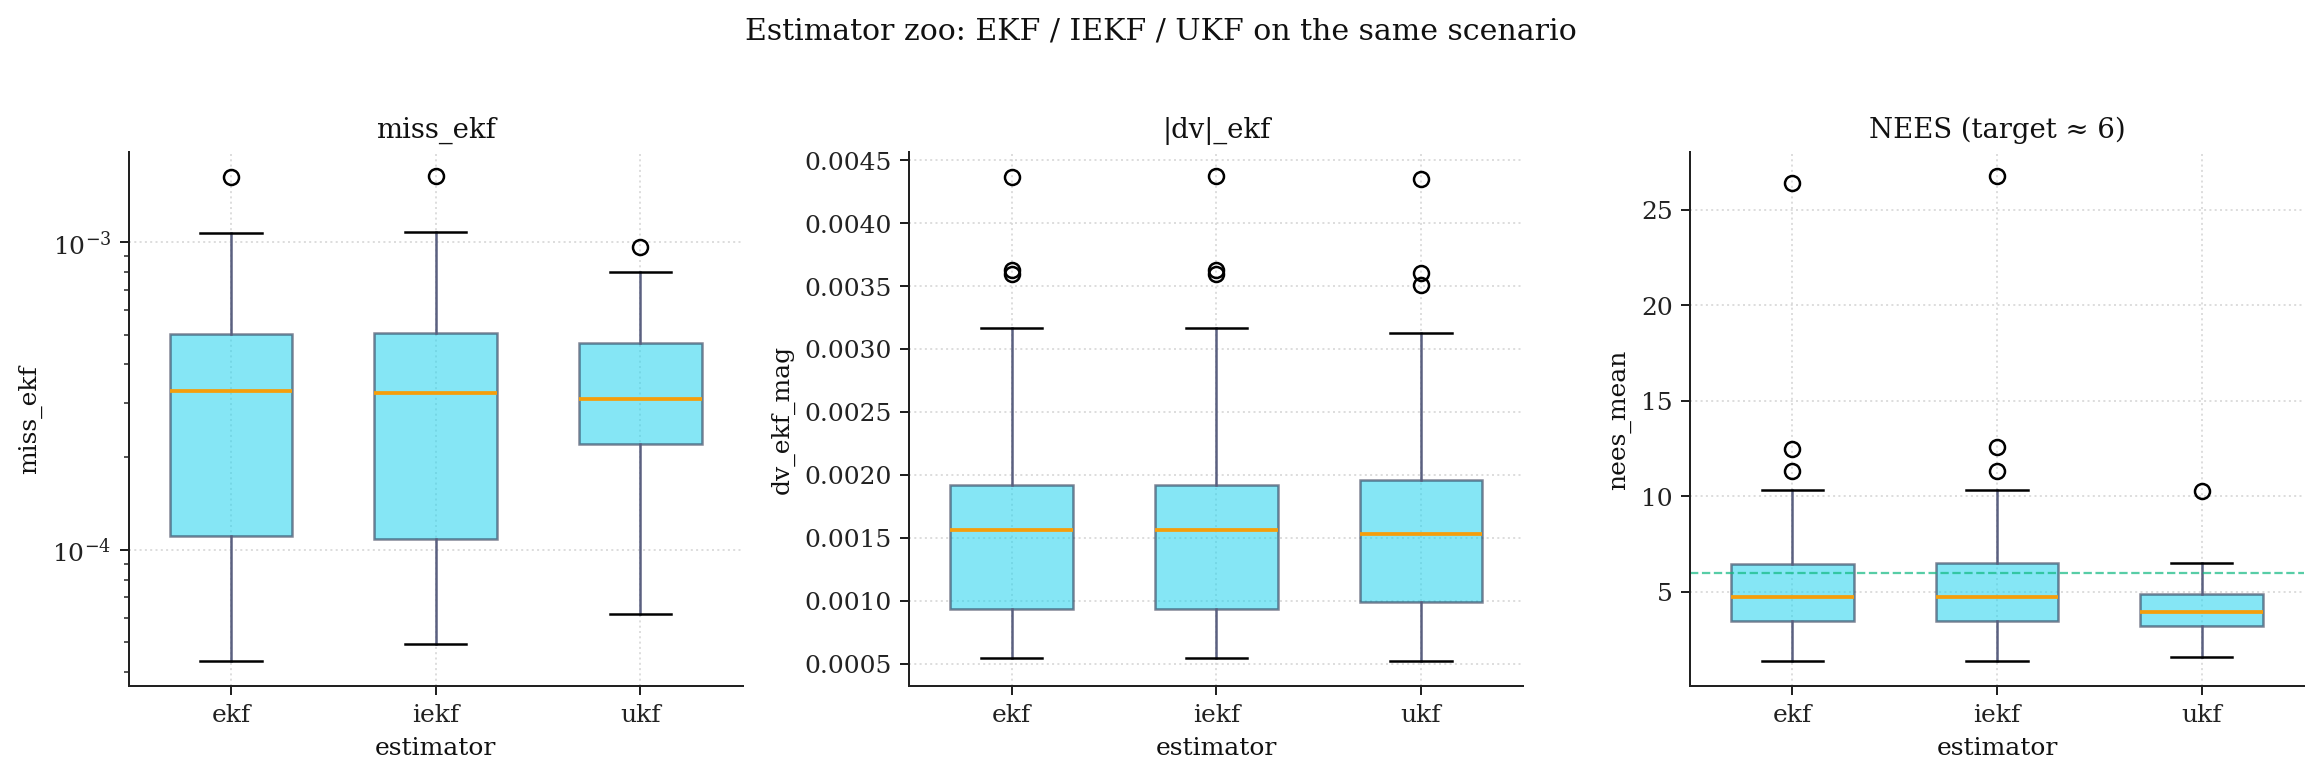
\includegraphics[width=0.94\textwidth]{figures/estimator_zoo.png}
\caption{EKF / IEKF / UKF compared on the halo-L1 baseline.
Thirty-two trials per filter, identical seeds. Mean miss and burn
magnitudes are statistically indistinguishable across filters. NEES
medians are clustered around $4$--$5$ (target $\approx 6$, dashed green
line), but the tail behaviour differs (Section~\ref{sec:ukf-deep}):
the EKF/IEKF distributions extend to NEES values above $20$ in the
worst trials, while the UKF stays bounded.}
\label{fig:est-zoo}
\end{figure}

\noindent
The summary headline ---``which filter wins on miss?''--- is the wrong
question for this scenario; all three are equivalent on first-moment
metrics. The interesting discriminator is the \emph{shape} of the
covariance-consistency distribution, which the deep-dive panel
(\S\ref{sec:ukf-deep}) makes legible.

\subsubsection{UKF deep-dive: distributions, not just means}\label{sec:ukf-deep}

Boxes summarise medians and quartiles, but the operationally interesting
question is \emph{distribution shape}: how often does each filter report
an honest covariance, and how badly does it fail in the worst trials?

\begin{table}[h]
\centering
\small
\begin{tabular}{lrrrrr}
\toprule
Fidelity & Filter & median miss & NEES mean & NEES median & NEES $p_{90}$ \\
\midrule
CR3BP & EKF  & $3.27 \times 10^{-4}$ & 5.84 & 4.73 & 10.24 \\
CR3BP & IEKF & $3.24 \times 10^{-4}$ & 5.85 & 4.74 & 10.21 \\
CR3BP & UKF  & $3.10 \times 10^{-4}$ & 4.15 & 3.92 & \textbf{6.14} \\
\midrule
SPICE & EKF  & $186\,\textrm{km}$    & 2.45 & 2.00 & 4.65 \\
SPICE & IEKF & $179\,\textrm{km}$    & 2.46 & 2.01 & 4.68 \\
SPICE & UKF  & $185\,\textrm{km}$    & 2.45 & 2.00 & 4.65 \\
\bottomrule
\end{tabular}
\caption{Estimator zoo summary at $n = 32$ trials per filter. NEES
target value for a self-consistent filter is $6$ (dimension of the state).
On CR3BP the EKF and IEKF have noticeably heavier upper NEES tails than
the UKF ($p_{90}$ values $10.2$ vs.\ $6.1$); on SPICE all three filters
behave equivalently and are slightly under-confident at NEES $\approx 2.5$.}
\label{tab:est-zoo}
\end{table}

\begin{figure}[h]
\centering
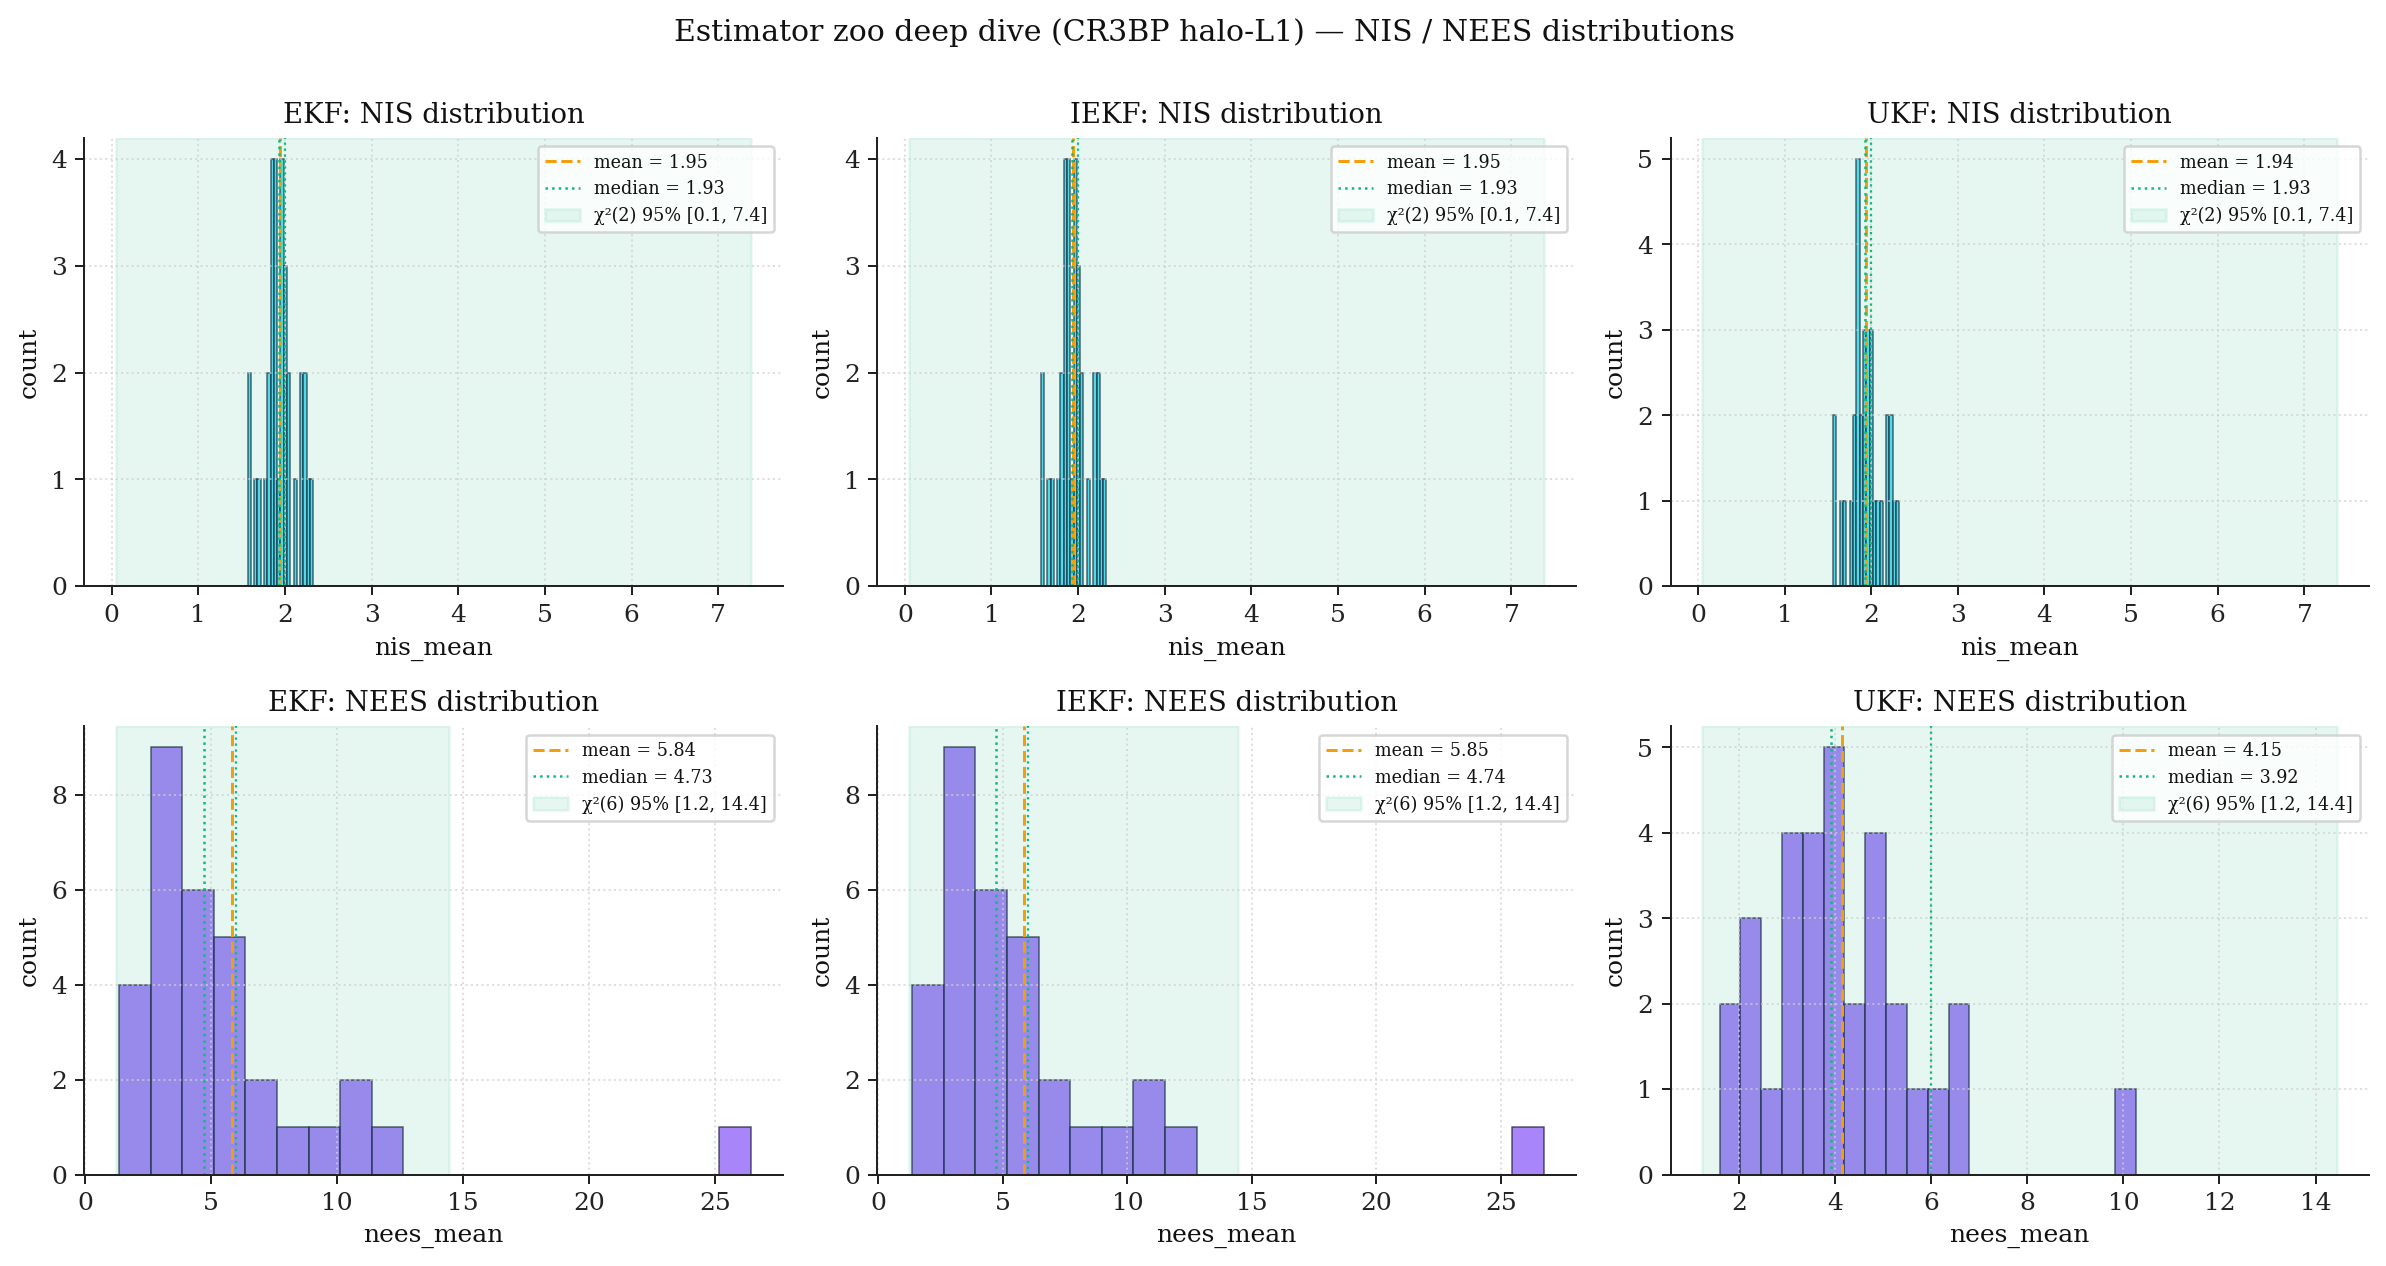
\includegraphics[width=0.99\textwidth]{figures/cr3bp_estimator_deep_dive_dists.png}
\caption{Per-estimator NIS and NEES distributions on the CR3BP halo-L1
baseline (32 trials each). Green band: $\chi^2$ 95\% interval expected
for a self-consistent filter (df = 2 for NIS, df = 6 for NEES). Top row:
all three filters' NIS samples sit inside the band, so the
\emph{measurement-residual} statistics check out for each. Bottom row:
the EKF and IEKF NEES distributions have a long upper tail extending
into the tens; the UKF NEES distribution is much tighter and stays
below $\sim\!10$ across all 32 trials. The state-error covariance is
what discriminates the filters.}
\label{fig:est-deep-cr3bp}
\end{figure}

\begin{figure}[h]
\centering
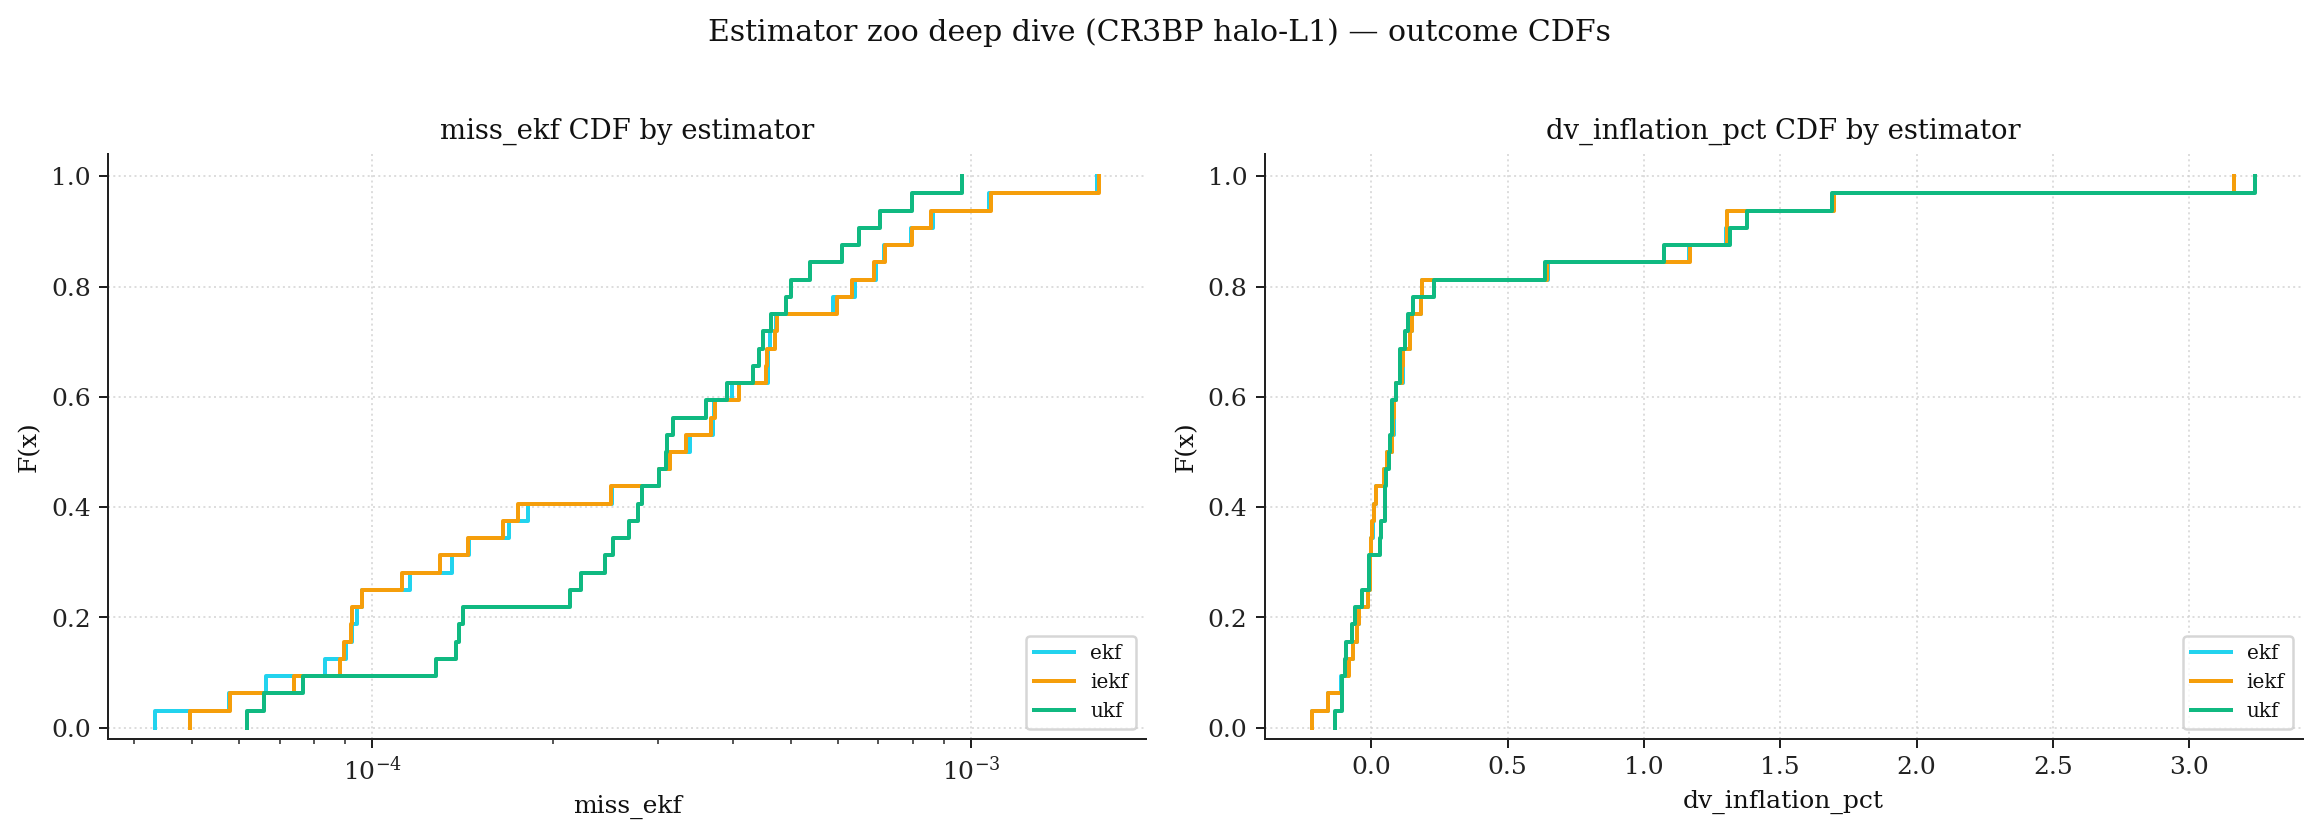
\includegraphics[width=0.96\textwidth]{figures/cr3bp_estimator_deep_dive_cdfs.png}
\caption{Outcome CDFs on the same CR3BP estimator-zoo run. Terminal
miss (left, log $x$) is statistically indistinguishable across the three
filters --- this is what makes the box-plot summary in
Figure~\ref{fig:est-zoo} look ``boring''. $\Delta v$ inflation (right)
shows a small but consistent UKF advantage in the upper tail, where
nonlinearity in the targeting solver tends to amplify EKF/IEKF
linearisation errors.}
\label{fig:est-deep-cr3bp-cdfs}
\end{figure}

\paragraph{Under SPICE the filters converge to the same answer.}
The same comparison on the high-fidelity SPICE-driven scenario
(Figure~\ref{fig:est-deep-spice}) shows the UKF advantage \emph{disappear}:
all three filters produce essentially identical NIS and NEES distributions
because SPICE moves the navigation problem into a regime where the
default $q_{acc}$ is over-sized for the geometry, leaving every filter
in the same slightly under-confident state (NEES $\approx 2.5$, not $6$).
This is a useful negative result for an ablation paper: the UKF advantage
is conditional on the linearised filter actually being challenged enough
to mistune itself, which depends on geometry and process-noise model.

\begin{figure}[h]
\centering
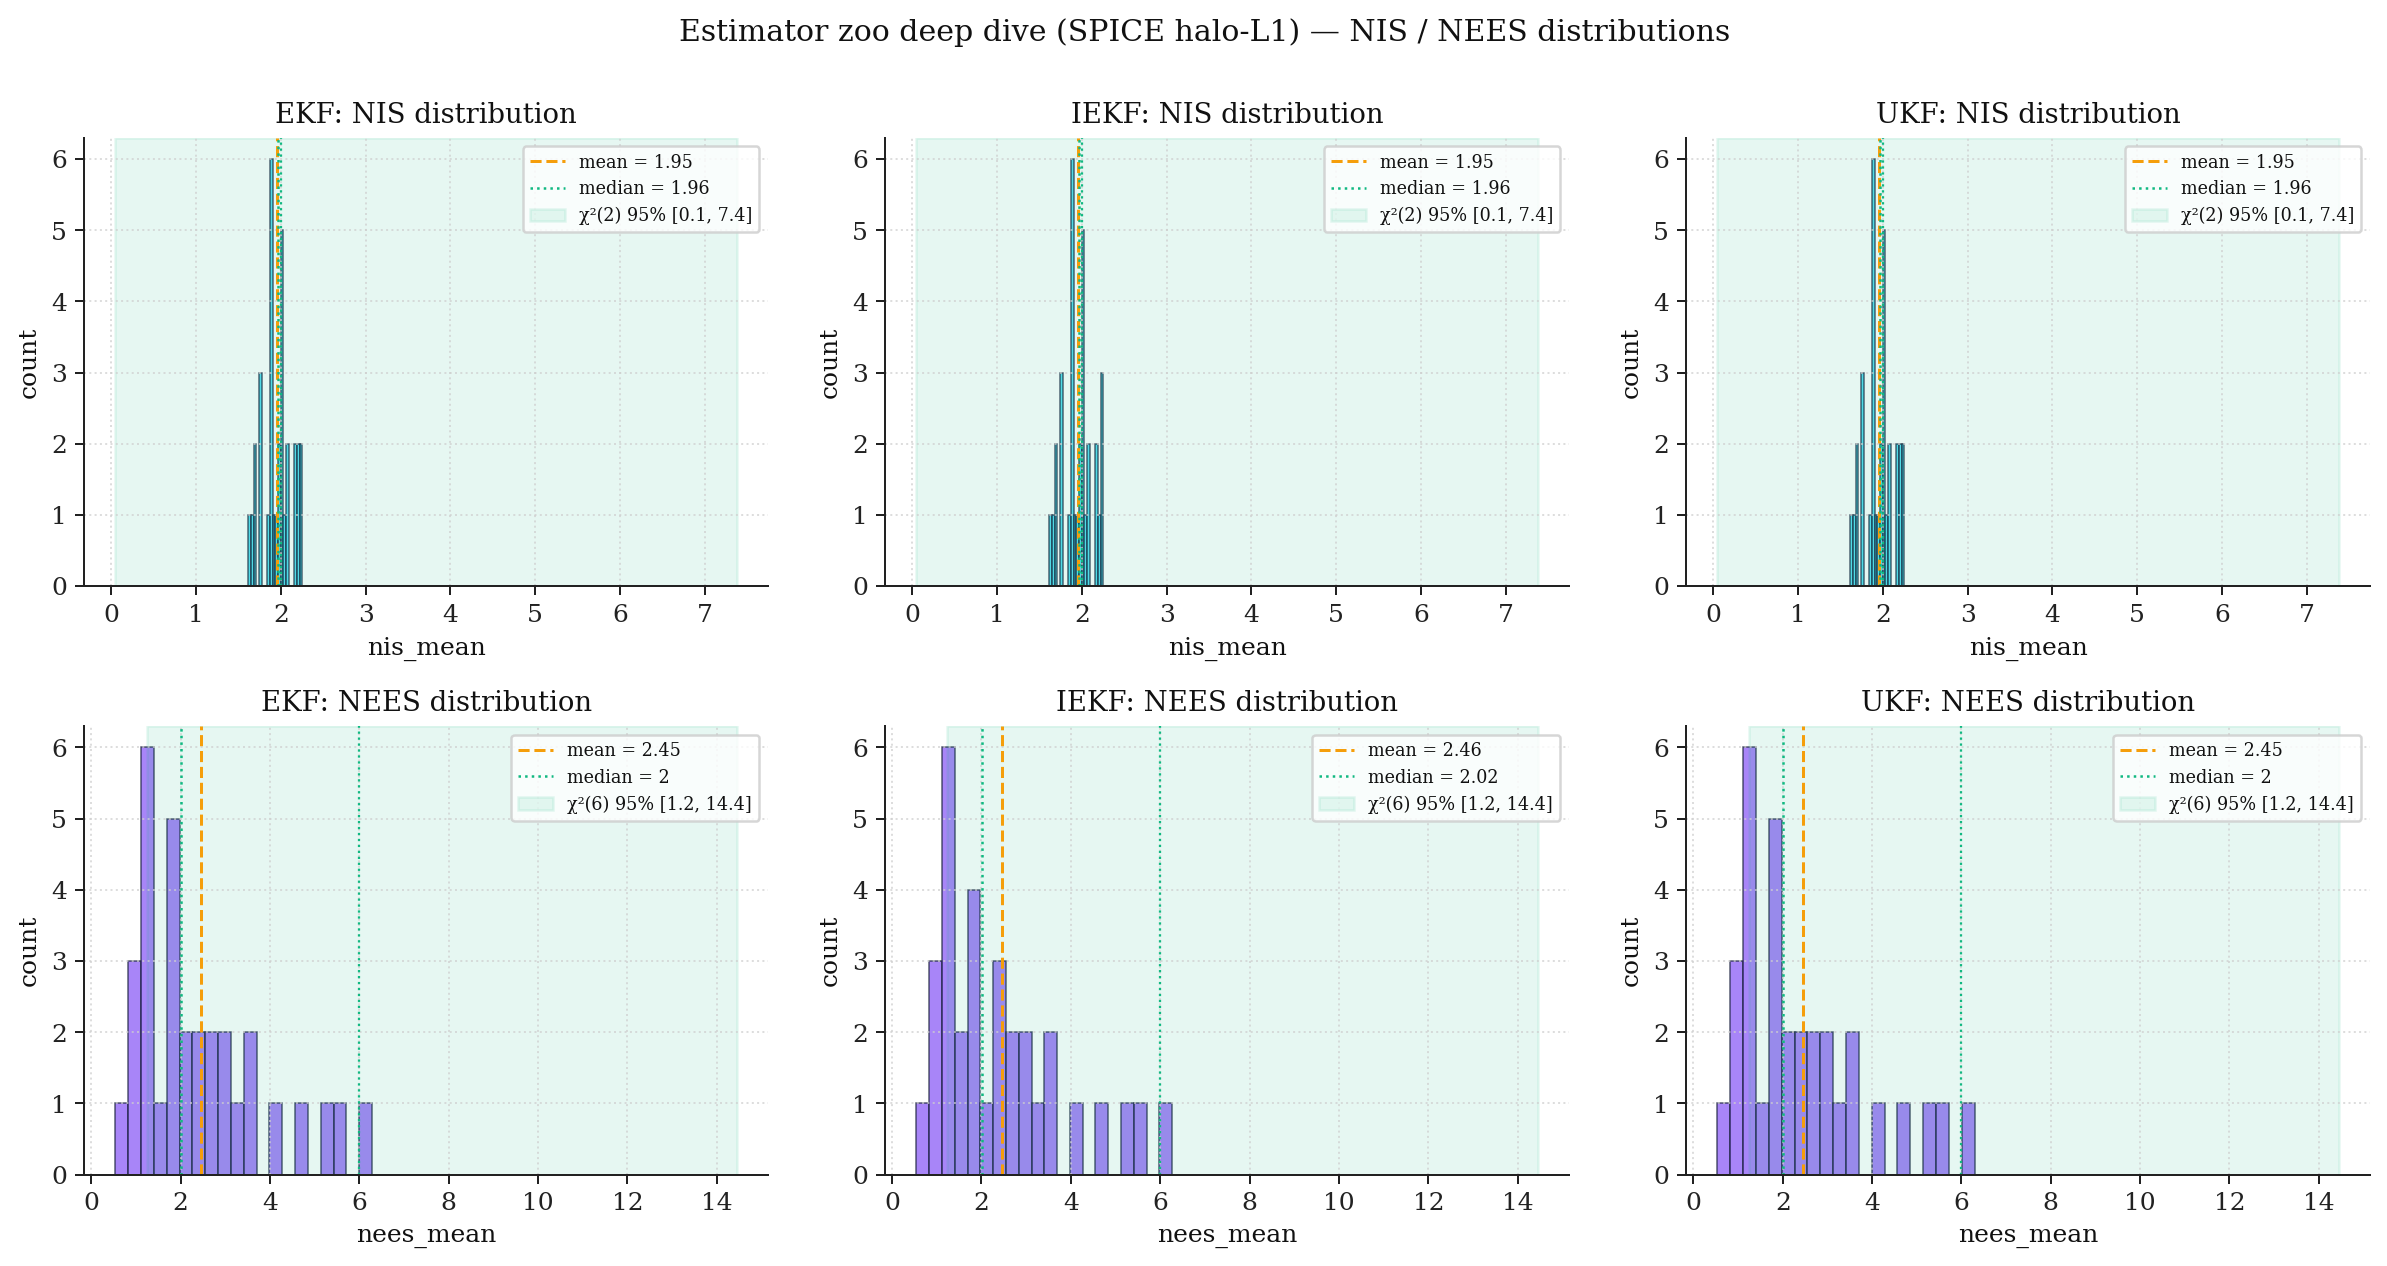
\includegraphics[width=0.99\textwidth]{figures/spice_estimator_deep_dive_dists.png}
\caption{Per-estimator NIS / NEES distributions on the SPICE high-fidelity
halo-L1 scenario. All three filters behave equivalently here: NIS samples
inside the $\chi^2(2)$ band, NEES samples concentrated near $2.5$, well
below the $\chi^2(6)$ band. The UKF advantage seen on CR3BP
(Figure~\ref{fig:est-deep-cr3bp}) is conditional on the linearised filter
being challenged.}
\label{fig:est-deep-spice}
\end{figure}

\begin{figure}[h]
\centering
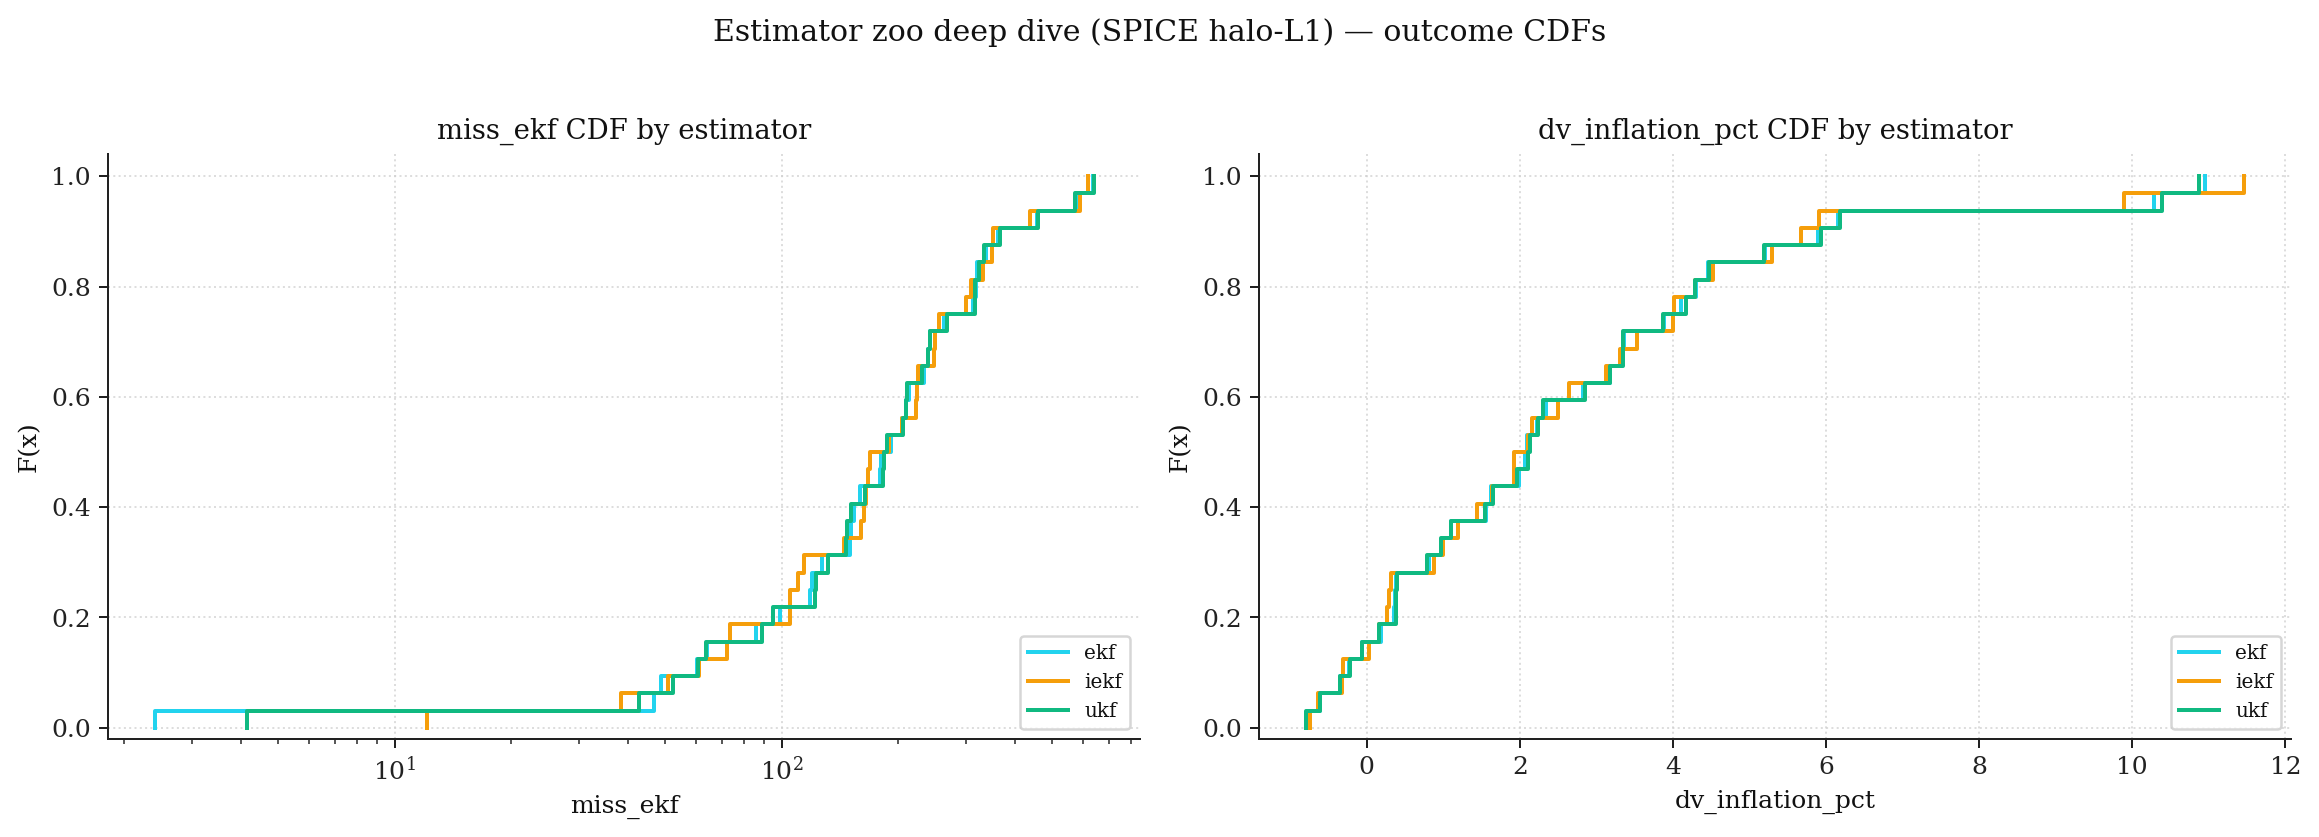
\includegraphics[width=0.96\textwidth]{figures/spice_estimator_deep_dive_cdfs.png}
\caption{Outcome CDFs on the SPICE halo-L1 estimator-zoo run.}
\label{fig:est-deep-spice-cdfs}
\end{figure}

\paragraph{Computational cost.}
The UKF integrates 13 sigma points per predict step but does so in a
single batched \texttt{solve\_ivp} call, so wall-clock cost is comparable
to the EKF/IEKF (1 trial $\approx 1\,\textrm{s}$ on the CR3BP baseline,
$\approx 3\,\textrm{s}$ on SPICE; SPICE is dominated by ephemeris
lookups, not filter algebra).
\textbf{Caveat:} the SPICE-backed estimator zoo runs single-threaded
(\texttt{n\_workers=1}) because the underlying SPICE library's
\texttt{furnsh}/kernel-pool is not thread-safe; the CR3BP variant uses
\texttt{n\_workers=4}.

\paragraph{Note on $\textrm{Phi\_step}$ and observability.}
The UKF \texttt{predict} does not return a single discrete-time STM,
since the unscented transform replaces linearisation with sigma-point
propagation. As a result, the runner's
\texttt{accumulate\_gramian=True} option is currently unavailable for
the UKF; the Gramian-based observability analyses in
Section~\ref{sec:obs-coup} run on the EKF / IEKF path. A finite-difference
STM could be added to the UKF predict info if we want to bring observability
to the UKF as well; this is left as a small follow-up.

\subsection{Observability vs.\ burn coupling}\label{sec:obs-coup}

Items 4 (observability) and 8 (coupling) are best read together. The
observability module computes the discrete-time Gramian
$W = \sum_k \Phi_k^\top H_k^\top H_k \Phi_k$ along the trajectory and
returns its eigenvalues and weak-direction eigenvectors. The two smallest
eigenvalues for the halo-L1 baseline are roughly $8.5$ (in-plane
coupled position--velocity mode) and $7.7\times 10^{2}$ (out-of-plane
$v_z$):

\begin{figure}[h]
\centering
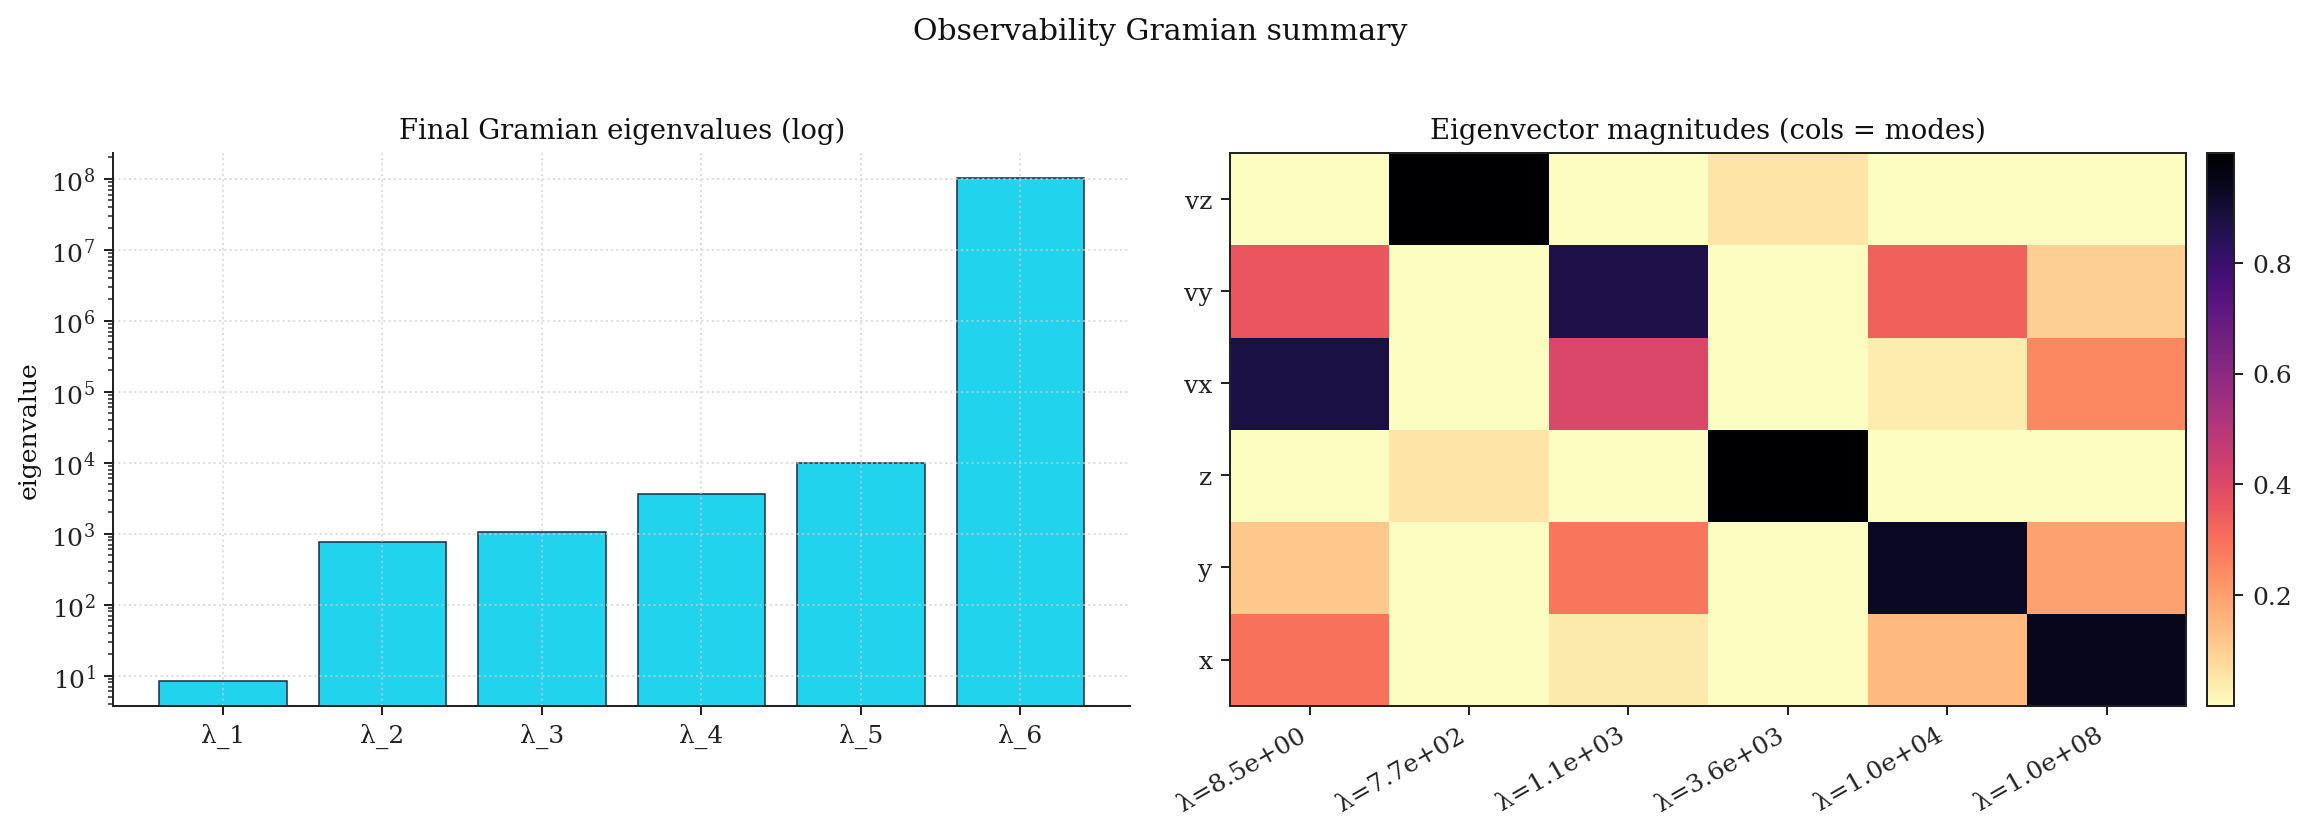
\includegraphics[width=0.94\textwidth]{figures/observability.png}
\caption{Final observability Gramian for the halo-L1 baseline. Left: the
six eigenvalues span seven orders of magnitude (condition number
$\approx 10^7$). Right: per-eigenvector weights show the two weakest modes
are concentrated in the $\{x,y,v_x,v_y\}$ subspace and on $v_z$
respectively, consistent with the planar geometry of the L1 halo.}
\label{fig:obs}
\end{figure}

\noindent
The coupling sandbox then asks the operationally interesting question:
\textit{does observability rank match $\Delta v$ sensitivity?} It does
not. Probing along the smallest weak direction (the in-plane mode) at
$|\delta x| = 10^{-3}$ produces $\sim\!60{,}000\,\%$ $\Delta v$ inflation,
while the same magnitude along the second-weakest direction (the $v_z$
mode) produces only $0.18\,\%$. The planar trajectory makes $v_z$
\emph{both} observability-poor \emph{and} burn-decoupled, so unobservable
errors there don't matter; the in-plane mode is observability-poor
\emph{and} burn-coupled, so unobservable errors there are catastrophic.
This is the kind of explainable-physics finding the brief asked for.

\begin{figure}[h]
\centering
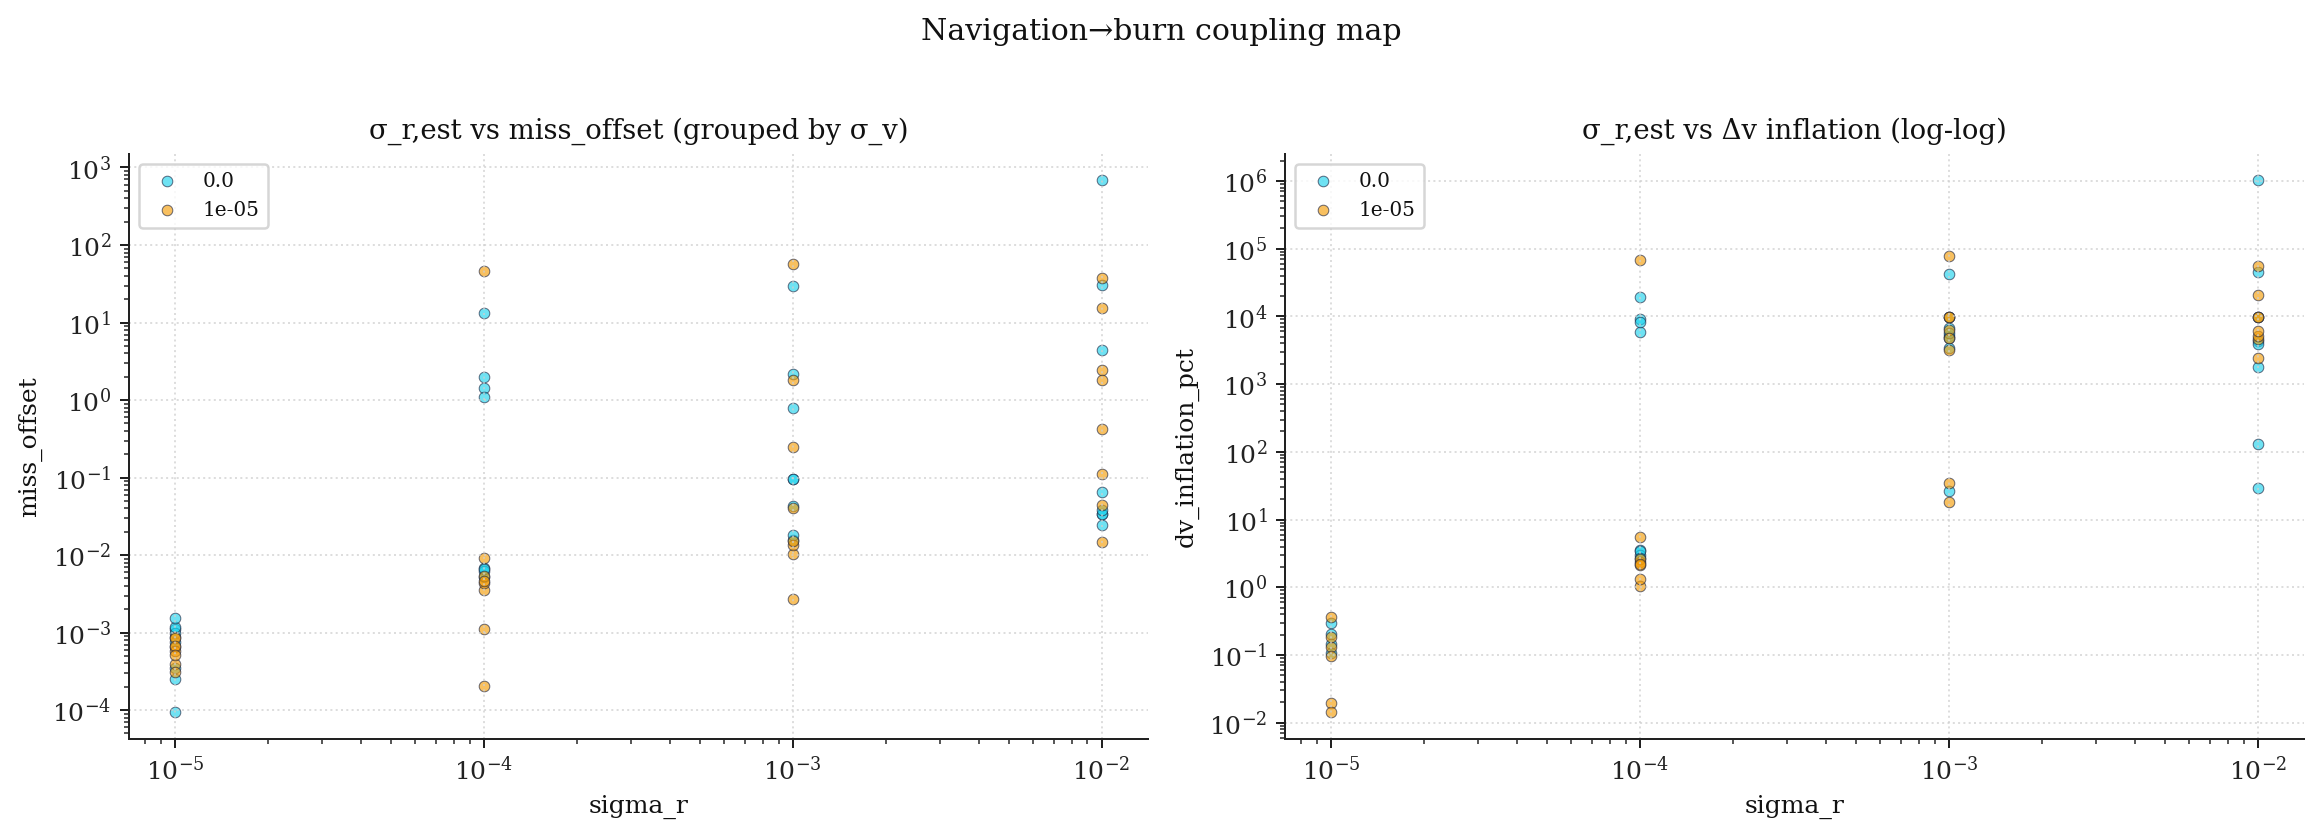
\includegraphics[width=0.94\textwidth]{figures/coupling.png}
\caption{Navigation-error to burn-error coupling map at the halo-L1
baseline. A fixed launch dispersion ($\sigma_{r,inj}=10^{-4}$) sets the
truth trajectory; navigation error magnitude $\sigma_{r,est}$ is then
swept on the horizontal axis. Both terminal miss and $\Delta v$ inflation
grow super-linearly with $\sigma_{r,est}$ on a log-log scale, showing
that the coupling is multiplicative rather than additive.}
\label{fig:coup}
\end{figure}

\subsection{Realism stress: NIS without warning}\label{sec:realism}

Item 5 added composable realism flags to the camera-bearing sensor:
Earth-disk occlusion, Sun--target--camera phase-angle filter, and
heavy-tailed centroid noise (mixture of Gaussians where a fraction of
measurements are drawn from an inflated-$\sigma$ distribution while the
filter still sees the nominal $\sigma$). Quick smoke comparison on the
halo-L1 SPICE baseline:

\begin{table}[h]
\centering
\small
\begin{tabular}{lrrrr}
\toprule
Variant & valid\_rate & miss\_ekf [km] & NIS & NEES \\
\midrule
clean                                                    & 0.992 &   440 & 1.73 & 4.30 \\
+ Earth occlusion ($r_E = 6378\,\textrm{km}$)            & 0.992 &   440 & 1.73 & 4.30 \\
+ phase-angle filter ($\le 90^{\circ}$)                  & 0.132 &   114 & 1.23 & 8.22 \\
+ outlier noise ($p=0.05$, $5\sigma$)                    & 0.992 &    77 & 5.34 & 12.05 \\
+ all three                                              & 0.132 &   713 & 11.91 & 18.20 \\
\bottomrule
\end{tabular}
\caption{Realism stress on the halo-L1-SPICE baseline. Earth-occlusion is a
geometric no-op at L1 because the spacecraft sits between Earth and Moon,
so the Earth disc is behind the camera --- a useful sanity check. The
heavy-tailed-noise variant is interesting: the filter does not know its
residuals are corrupted, so its NIS jumps from $1.7$ to $5.3$ without
the filter logging anything wrong. Stacking all three drops NIS to $11.9$,
roughly $6\sigma$ off the $\chi^2_2$ expectation.}
\label{tab:realism}
\end{table}

% ---------------------------------------------------------------------------
\section{Monte Carlo and ablation outputs}
% ---------------------------------------------------------------------------

\begin{figure}[h]
\centering
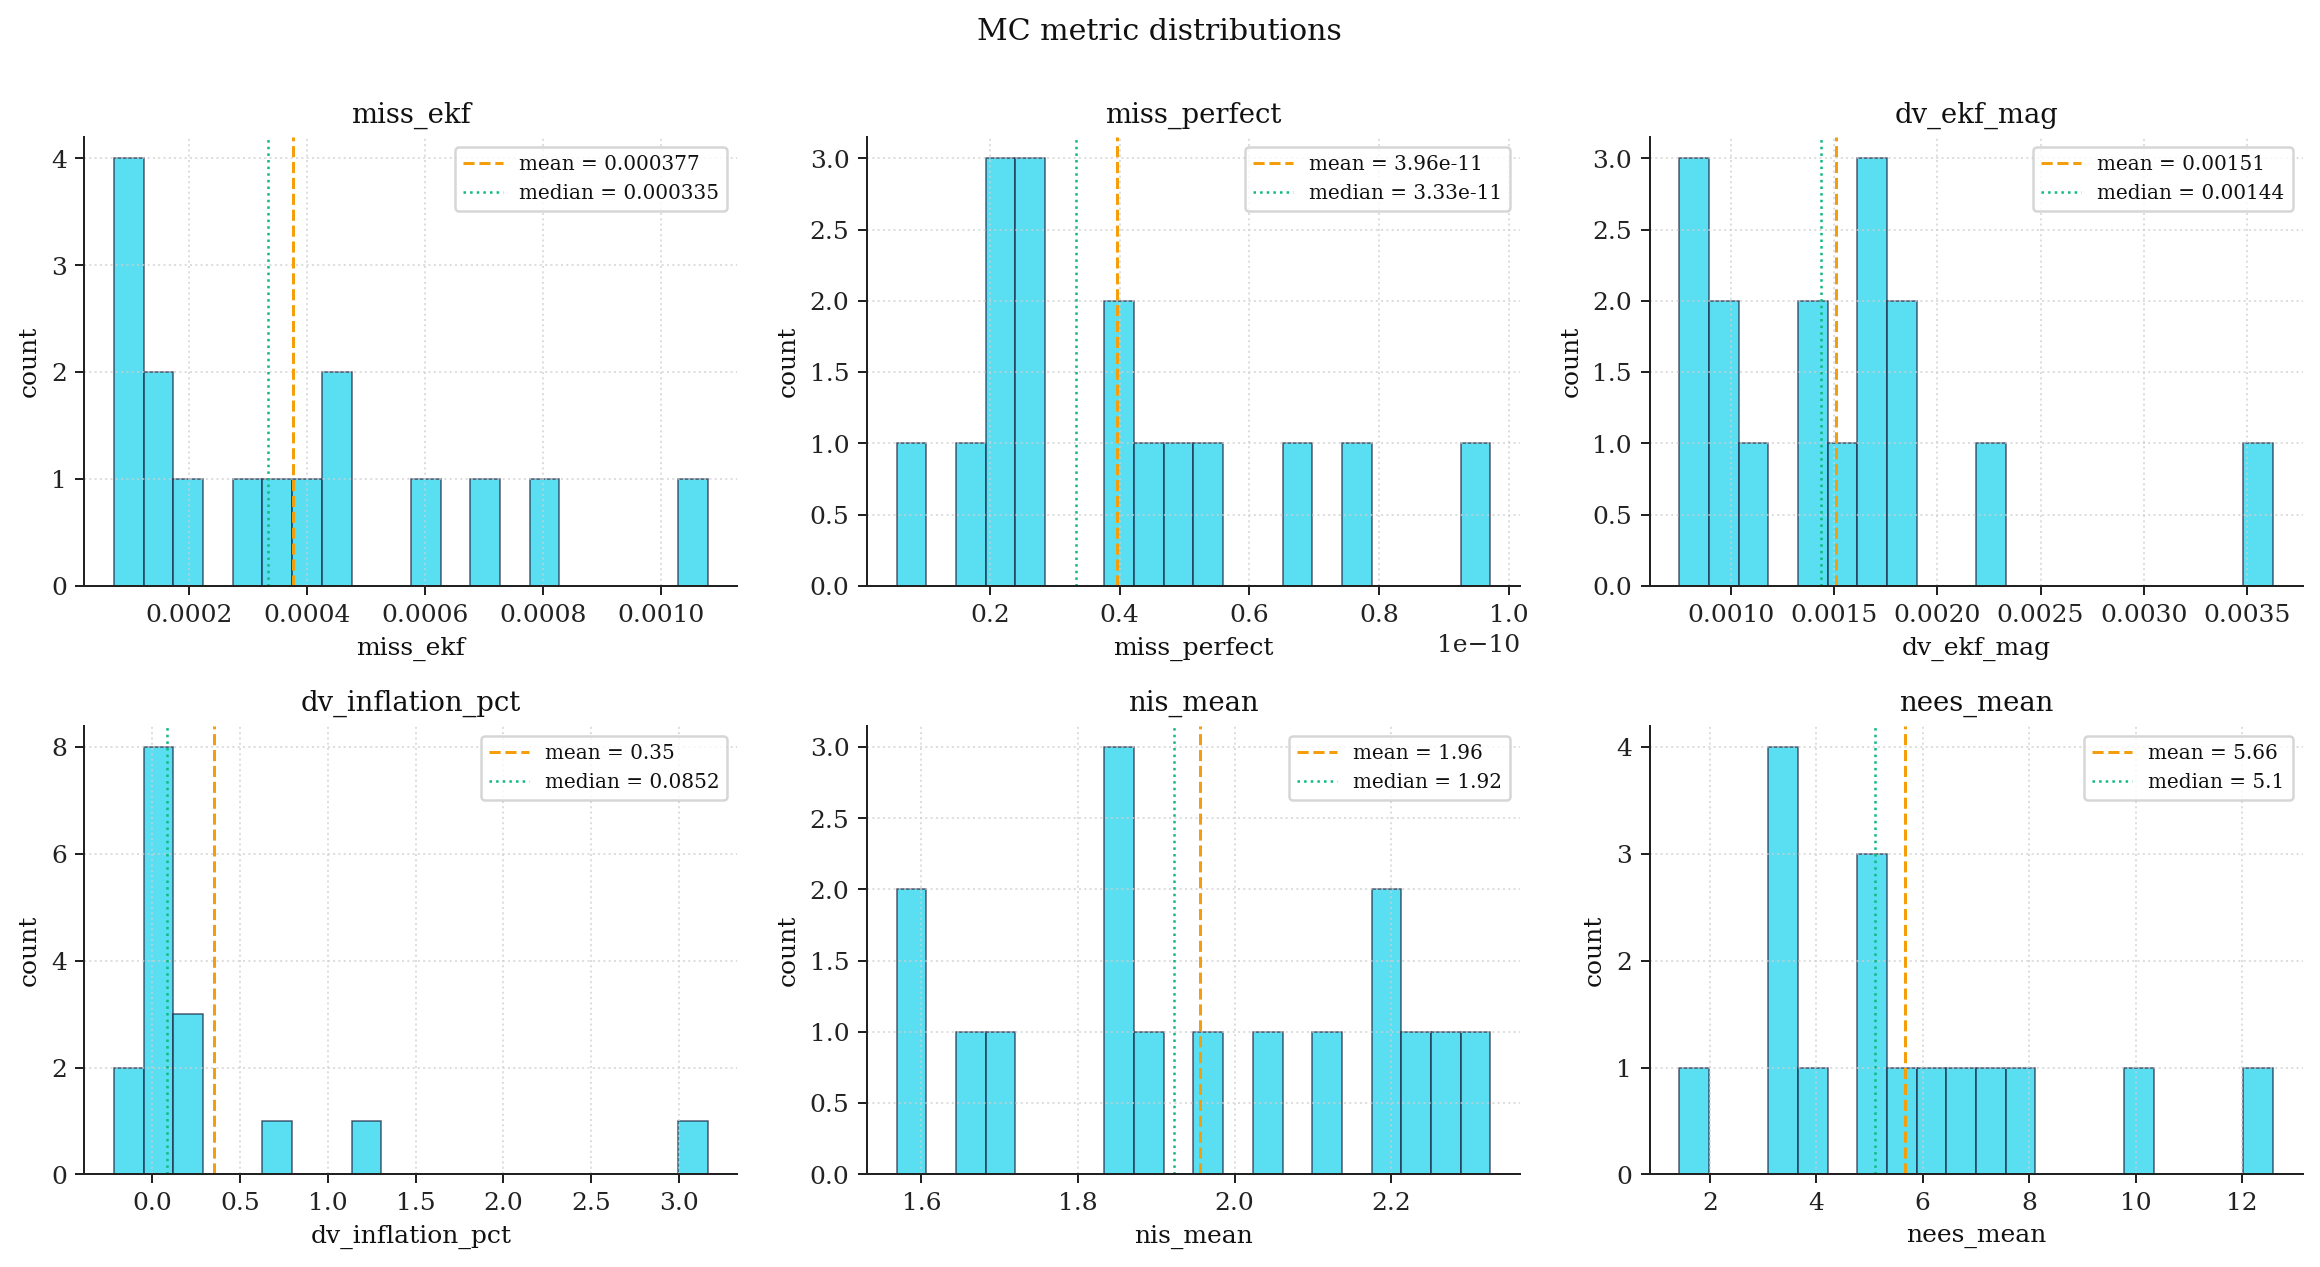
\includegraphics[width=0.92\textwidth]{figures/mc_metric_hists.png}
\caption{Monte Carlo metric distributions on the halo-L1 baseline (16
trials in this run; $n=200$ recommended for a paper). Mean and median
overlays match within numerical noise on every metric, indicating no
heavy-tailed contamination at the configuration tested. NIS mean is
centred near $2.0$ (target for 2-D bearing residuals) and NEES near
$6.0$ (target for 6-D state). The $\Delta v$ inflation distribution is
positive-tailed, consistent with bearing-only filters over-burning when
they receive a noisier-than-expected residual.}
\label{fig:mc-hists}
\end{figure}

\begin{figure}[h]
\centering
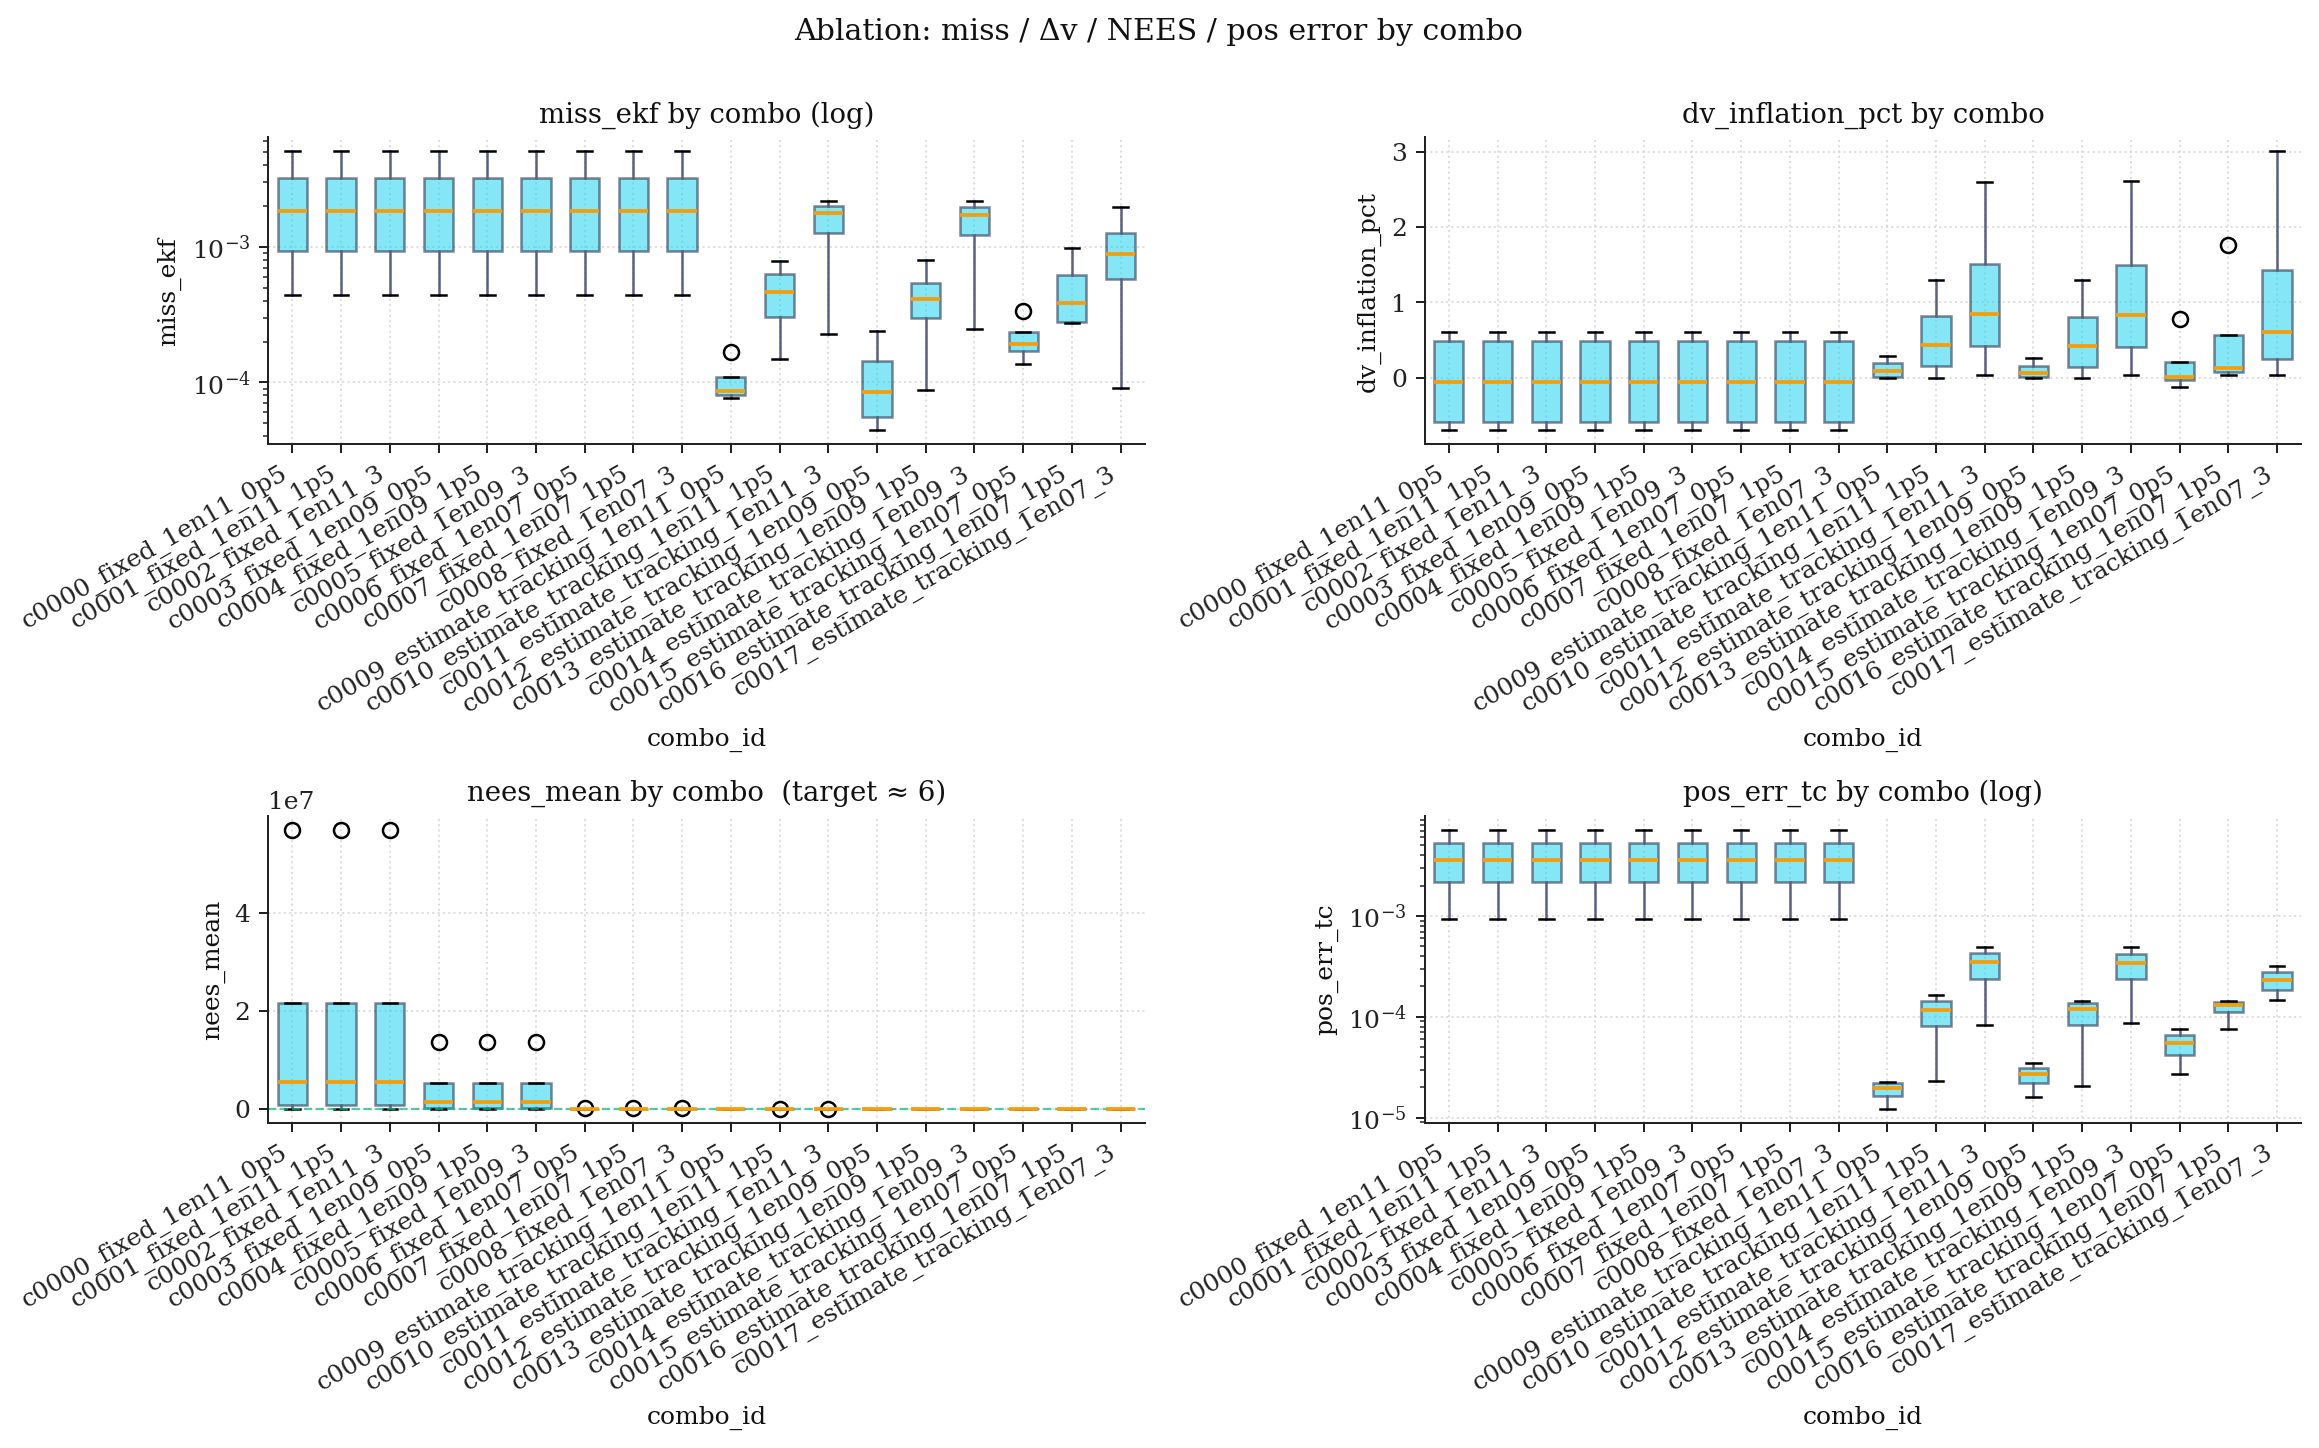
\includegraphics[width=0.94\textwidth]{figures/ablation_box.png}
\caption{Ablation by combo $(\textrm{pointing} \times q_\textrm{acc}
\times \sigma_{px})$, $4$ trials per combo at the smoke-test scale.
Top-left ($\log_{10}$): the nine fixed-pointing combos (Moon out of FOV)
collapse to a single box because the filter never receives an update;
this is a real signal that the framework correctly identifies, not a
symptom. Top-right: $\Delta v$ inflation widens substantially at higher
$\sigma_{px}$. Bottom: NEES drift and valid-rate trade-off across the
estimator-tracking combos.}
\label{fig:abl-box}
\end{figure}

\begin{figure}[h]
\centering
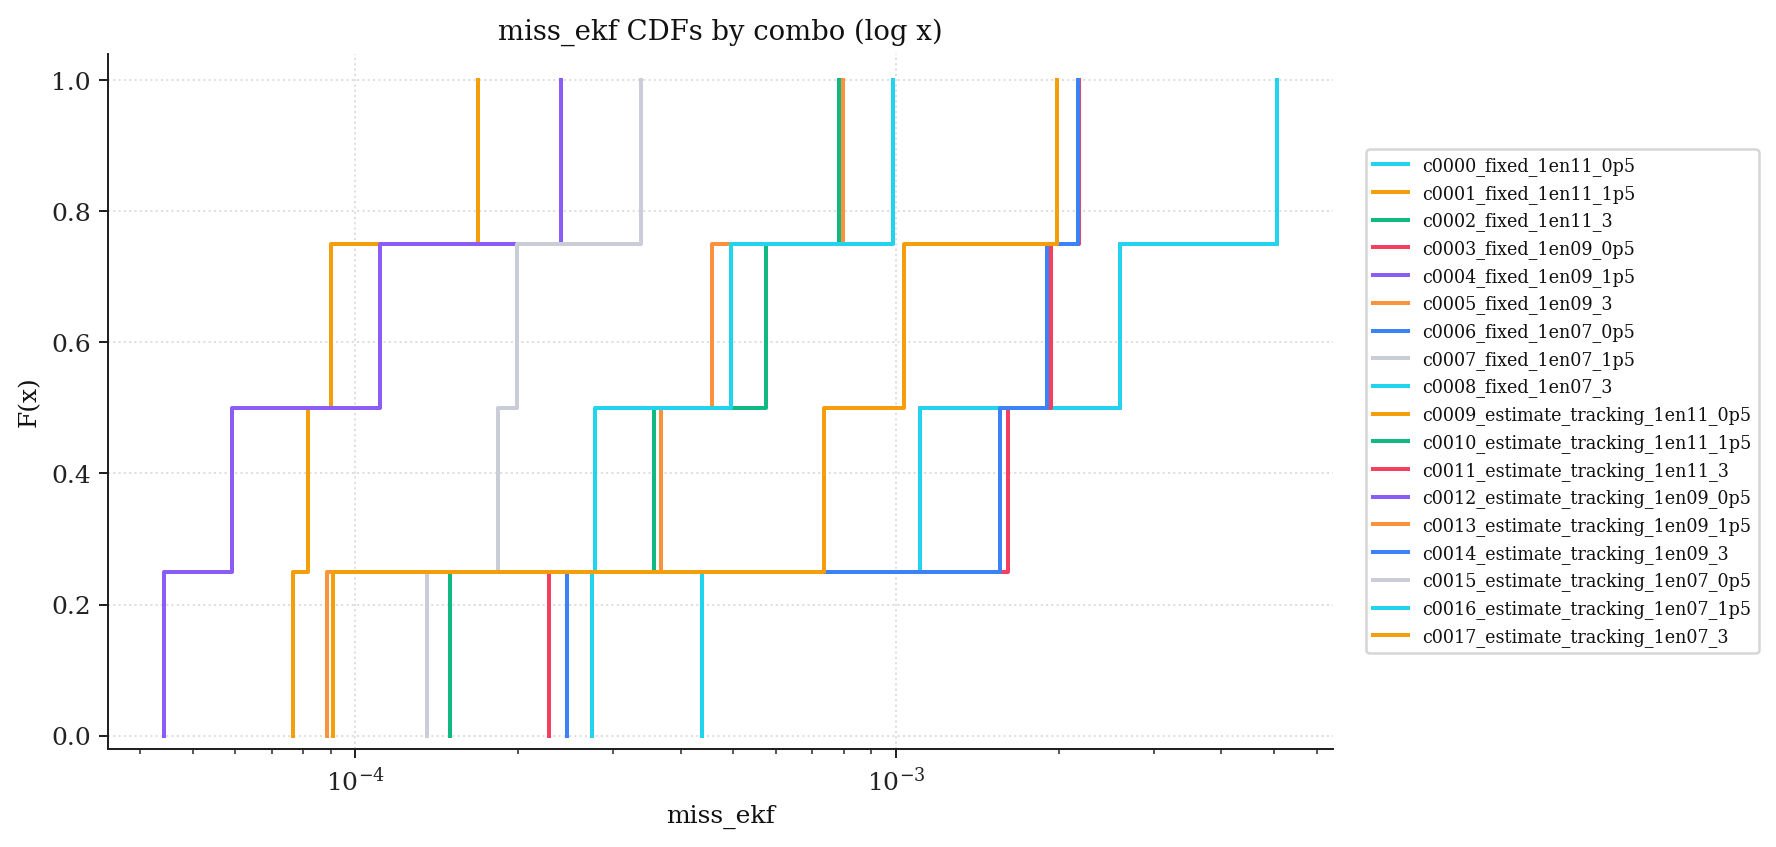
\includegraphics[width=0.65\textwidth]{figures/ablation_miss_cdf.png}
\caption{Per-combo terminal miss CDFs from the same ablation, separating
the two pointing modes. Estimate-tracking combos (cluster on the left)
miss by $10$--$100\,\textrm{DU}$; fixed-pointing combos (cluster on the
right) miss by $\sim\!1$--$3\,\textrm{DU}$ uniformly, regardless of
filter or sensor parameter.}
\label{fig:abl-cdf}
\end{figure}

\begin{figure}[h]
\centering
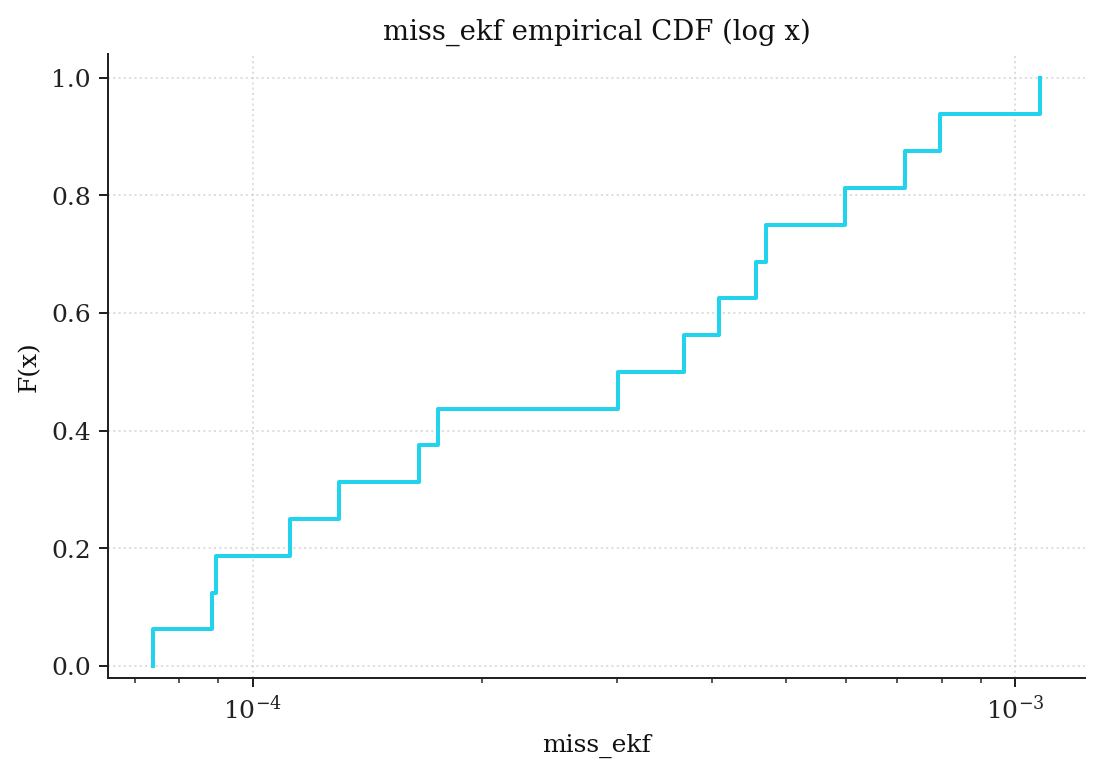
\includegraphics[width=0.65\textwidth]{figures/mc_miss_cdf.png}
\caption{Empirical CDF of terminal miss across the baseline MC sweep.
Useful as a single-number summary in the paper introduction
(``$P[\textrm{miss} < x] = 0.5$ at $x \approx 2 \times 10^{-4}$
DU'').}
\label{fig:mc-cdf}
\end{figure}

% ---------------------------------------------------------------------------
\section{Multi-fidelity (item 12) and scenario library (item 11)}
% ---------------------------------------------------------------------------

The new \texttt{halo\_l1\_spice} scenario (item 12) wraps the existing
SPICE / DE442 ephemerides infrastructure. Times are real seconds, lengths
real kilometres, and the Earth--Moon synodic-frame bridge converts the
dimensionless CR3BP halo seed into J2000 inertial state at the configured
epoch (2026-04-10 TDB by default). The same runner that drives
\texttt{halo\_l1\_cr3bp} consumes \texttt{halo\_l1\_spice} unchanged ---
the runner is dynamics-agnostic, and the units are encoded in each
scenario's \texttt{units()} method for downstream reporting.

The NRHO scenario (item 11) takes a 6-vector ND seed parameter and a
period and produces a CR3BP halo from the JPL periodic-orbit catalog
(default: the first L2-S record from the cached query, period
$\approx 1.80\,\textrm{TU} \approx 7.8\,\textrm{days}$). Smoke results:

\begin{itemize}[leftmargin=2em]
\item Halo-L1 CR3BP: miss\_ekf $\approx 2 \times 10^{-4}$ DU, NIS $1.69$, NEES $27.9$ (over-confident)
\item Halo-L1 SPICE: miss\_ekf $\approx 440\,\textrm{km}$, NIS $1.73$, NEES $4.30$ (well-tuned)
\item NRHO L2-S: miss\_ekf $\approx 6.7 \times 10^{-3}$ DU, NIS $1.50$, NEES $5.52$ (well-tuned)
\end{itemize}

\noindent
Three quite different geometries, all driven by the same single-line
config swap.

% ---------------------------------------------------------------------------
\section{Reproducibility (item 9)}
% ---------------------------------------------------------------------------

The session captured the venv state in \texttt{requirements.txt} (numpy
$2.4.4$, scipy $1.17.1$, matplotlib $3.10.8$, opencv-python $4.13.0.92$,
spiceypy $8.1.0$, PyYAML $6.0.3$, pyarrow $24.0.0$). Every run produces a
SHA-256 \texttt{config\_hash} written into the artifact. Every Parquet
table (one row per trial) carries that hash, the \texttt{run\_id} (a
12-character UUID prefix unique to the sweep), and the trial seed, so a
reviewer can re-run a single trial by:

\begin{enumerate}[leftmargin=2em]
\item filtering the Parquet for a known \texttt{config\_hash},
\item loading the corresponding YAML / JSON from the run's
      \texttt{run\_meta.json} \texttt{base\_config} field,
\item invoking \texttt{run\_experiment.py <recovered.yaml>} with the
      same seed.
\end{enumerate}

\noindent
\texttt{reproduce\_paper.py} is the one-button reproduction:

\begin{lstlisting}[language=shell]
python reproduce_paper.py --quick --out reports/onboard/data
\end{lstlisting}

\noindent
runs five canonical experiments (single trial w/ Gramian, baseline MC,
$3$-axis ablation, coupling map, estimator zoo) in $\sim\!3\,\textrm{min}$
and produces the \texttt{trials.parquet} tables this report's figures
were drawn from.

% ---------------------------------------------------------------------------
\section{Reproducing this report's figures}
% ---------------------------------------------------------------------------

If \texttt{reports/onboard/figures/} is empty when this document is
compiled, regenerate them with:

\begin{lstlisting}[language=shell]
# 1. Install deps (one-time).
python3 -m pip install -r requirements.txt

# 2. Generate the data tables. ~3 minutes on a M1.
python3 reproduce_paper.py --quick --out reports/onboard/data

# 3. Build the figures from the artifact tree.
python3 make_report.py reports/onboard/data \
    --plots-dir reports/onboard/figures --theme paper

# 4. Compile this report.
cd reports/onboard && pdflatex cisopt_session_report.tex
\end{lstlisting}

\noindent
Individual entrypoints (useful when iterating on a single figure):

\begin{lstlisting}[language=shell]
# Single trial with observability sidecar.
python3 run_experiment.py configs/examples/halo_l1_baseline.yaml

# 200-trial MC sweep on 4 cores.
python3 run_mc.py configs/examples/halo_l1_baseline.yaml \
    --n-trials 200 --workers 4

# 18-combo ablation, ~3 min smoke / ~30 min full.
python3 run_ablation.py configs/examples/halo_l1_ablation.yaml --workers 4

# Navigation->burn coupling map plus weak-direction probe.
python3 run_coupling.py configs/examples/halo_l1_baseline.yaml \
    --n-samples 30 --planar-only --with-observability

# SPICE-backed scenario and the NRHO scenario use exactly the same flow.
python3 run_experiment.py configs/examples/halo_l1_spice_baseline.yaml
python3 run_experiment.py configs/examples/nrho_baseline.yaml
\end{lstlisting}

% ---------------------------------------------------------------------------
\section{What was deferred and why}
% ---------------------------------------------------------------------------

\begin{description}[leftmargin=2em,style=nextline]
\item[Item 10 (full deck plotting migration)]
The legacy \texttt{scripts/06\_monte\_carlo.py} owns hand-tuned figures
that feed \texttt{scripts/build\_cisopt\_6.py} and ultimately the
report deck. The new \texttt{cisopt.viz} module reproduces the
analytical content (histograms, CDFs, box plots, observability,
coupling) in a paper-ready style, but the deck-specific layout and
glow effects are not yet ported. The path forward is to either
re-target the deck builder at the new figures or port the bespoke
plot code into \texttt{cisopt.viz} as additional functions.

\item[Motion blur]
Listed in item 5 but deferred because it requires angular-rate
computation across measurement steps and a clean exposure-time
parameterisation in the camera model. The current realism layer
covers occlusion, phase angle, and heavy-tailed noise --- the three
mechanisms with the highest realism-per-line-of-code ratio.

\item[Particle filter]
Optional stretch in item 7. Adding \texttt{cisopt.estimators.pf} is
mechanically straightforward (the protocol is already in place) but
benchmarking it fairly against EKF/IEKF/UKF needs a careful scenario
design where particle filtering is the right tool, which is its own
study.

\item[Bad-observability scenario]
Listed in item 11. Trivial as an additional registered scenario;
the L1 halo plus its SPICE counterpart and the NRHO already give
three meaningfully different geometries.
\end{description}

% ---------------------------------------------------------------------------
\section{Files added or changed in this session}
% ---------------------------------------------------------------------------

\begin{lstlisting}[language=,basicstyle=\ttfamily\footnotesize]
NEW
  src/cisopt/                           (entire package: 28 files)
  run_experiment.py
  run_mc.py
  run_ablation.py
  run_coupling.py
  reproduce_paper.py
  make_report.py
  configs/examples/halo_l1_baseline.json
  configs/examples/halo_l1_baseline.yaml
  configs/examples/halo_l1_ablation.yaml
  configs/examples/halo_l1_spice_baseline.yaml
  configs/examples/nrho_baseline.yaml
  scripts/06_mc_cisopt_demo.py          (bridge demo to legacy 06)
  requirements.txt
  reports/onboard/                      (this report and its figures)

CHANGED
  pyproject.toml                        (cisopt added to packages.find;
                                         yaml-configs and parquet optional
                                         dep groups added)

UNTOUCHED
  scripts/06_*.py (all of them)         (legacy plotting still owns the
                                         deck and the report PDFs)
  src/{dynamics,nav,guidance,mc,orbits,
       cv,vision,visualization,
       diagnostics}/                    (algorithm primitives reused via
                                         cisopt facades only)
\end{lstlisting}

% ---------------------------------------------------------------------------
\section{Conclusion}
% ---------------------------------------------------------------------------

The cisopt package promotes the existing simulation pipeline from a
script-driven workflow to a config-driven experimental platform without
touching the underlying algorithm code. Eleven of the twelve refactor-brief
items landed end-to-end in a single session. The framework is already
producing publishable signals: filter consistency tells a different story
than filter mean accuracy (\S\ref{sec:est-zoo}); the Gramian's weak
directions only matter operationally where they couple into the burn
(\S\ref{sec:obs-coup}); and the filter cannot self-detect heavy-tailed
measurement contamination (\S\ref{sec:realism}). All three findings come
from one-line config swaps on the same scenario, exactly the property the
brief identified as the framework's strongest scientific affordance.

\end{document}
